\chapter{Gerelateerd Werk}
\label{hoofdstuk:related}
Het automatisch genereren van beschrijvingen voor ongeziene afbeeldingen is een complex proces. Het combineert zowel computervisie (CV) als natuurlijke taalverwerking (NLP). Vele modellen zijn al voorgesteld die telkens elementen uit beide onderzoeksvelden combineren. Daarom volgt er eerst een opdeling van de gerelateerde literatuur op basis van de gebruikte technieken in deze twee domeinen. 

Dit onderzoeksdomein werd eerst niet beschouwd als generatieprobleem maar als opvraag- of retrievalprobleem. Hierbij zoekt een model naar de beste zin in een bestaande verzameling van zinnen op basis van de ingevoerde foto.\cite{Hodosh2013} Andere papers behandelen het probleem als een vertalingsprobleem naar analogie met automatisch vertalen. Hierbij gebruikt men een encoder-decoder framework waarbij de afbeelding als brontaal wordt beschouwd en het Engels als doeltaal.

Dit hoofdstuk bevat een overzicht van de gebruikte technologie uit computervisie en NLP voor het genereren van beschrijvingen. Daarnaast bespreken we de verschillende manieren waarop deze technologi\"en in de literatuur ge\"integreerd worden in \'e\'en model.

\section{Representatie van afbeeldingen}
Alle huidige modellen gebruiken technieken uit computervisie om nuttige features af te leiden uit afbeeldingen. Features bevatten onder andere gedetecteerde acties, sc\`enes en objecten met hun attributen en relaties.\cite{Bernardi} Deze features vormen de basis voor een representatie van de afbeelding die als input dient voor het generatie (of retrieval) model. 

Eerst volgt een bespreking van technieken die in het verleden zijn gebruikt. Daarna volgt een beschrijving van Convolutionele Neurale Netwerken (CNN), die in de meer recente literatuur veelvuldig voorkomen.


\subsection{Oorspronkelijke CV modellen}
De literatuur gebruikt meerdere technieken uit computervisie om nuttige features of eigenschappen af te leiden uit afbeeldingen. Features die in de vroegste papers over dit onderwerp voorkomen zijn bijvoorbeeld sc\`ene classificaties, object detecties en attribuut classifiers \cite{Farhadi2010,Yang2011,Patterson2014}. Concreet traint men modellen om voor elke afbeelding een bepaalde sc\`ene (bvb. restaurant, slaapkamer, keuken) af te leiden. 

Ook modellen die verschillende objecten detecteren en benoemen zijn hier van nut. Van zulke gevonden objecten kunnen classifiers ook nog nuttige attributen zoals kleur afleiden. Om zulke voorspellingen te doen gebruiken verschillende oudere papers bestaande classifiers en detectors zoals \cite{Felzenszwalb2008} Im2Text \cite{Ordonez2011} en GIST \cite{Oliva2006}. Ee\'n of meerdere van deze features kan dan rechtstreeks de representatie vormen van een afbeelding. Daarnaast vormen deze features in enkele werken \cite{Farhadi2010,Yang2011,Li2011,Mitchell2012} enkel de input voor abstracte afbeeldingsrepresentaties in de vorm van tupels. Deze tupels bevatten dan objecten, acties tussen objecten, sc\`ene types en/of ruimtelijke relaties.

Een andere manier om afbeeldingen te representeren is het gebruik van Visual Dependency Representations (VDR) zoals voorgesteld door \cite{Elliott2013}. Dit model werkt naar analogie met een afhankelijkheidsgrammatica in de taal. VDR's gebruiken een afhankelijkheidsgraaf om de ruimtelijke relaties tussen de objecten in een foto voor te stellen. Elke relatie tussen twee objecten krijgt dan een ruimtelijk positie als label. Mogelijke relaties zijn bijvoorbeeld \texttt{op, boven, onder, naast, ...} Het leren van VDR's kan op basis van geannoteerde training data, automatisch met objectherkenning \cite{Elliott2015} of nog met andere informatie die in de abstracte sc\`ene zit. \cite{Gilberto2015} 

\subsection{CV met behulp van neurale netwerken}
Naast deze meer traditionele manieren om informatie uit afbeeldingen af te leiden, bieden neurale netwerken een alternatieve oplossing.
Voor de meeste taken binnen computervisie blijkt dat convolutionele neurale netwerken (CNN) beter presteren dan bovenstaande methodes. Deze CNNs zijn deep learning neurale netwerken met soms meer dan 15 verborgen lagen. CNN's hebben minder verbindingen en parameters dan overeenkomstige feedforward neurale netwerken terwijl ze niet veel slechter presteren.\cite{Krizhevsky2012} 
Voor verschillende CV-taken werken de huidige state-of-the-art oplossingen op basis van CNN's. Dit is onder andere het geval voor gezichtsherkenning \cite{Zhou2015}, tekenherkenning \cite{Ciresan2012} en objectherkenning\cite{Szegedy2014}.

De gebruikte CNN's binnen het automatisch afbeeldingen beschrijven zijn netwerken die getraind zijn op ImageNet.\cite{Russakovsky2014} ImageNet is een dataset bestaande uit miljoenen afbeeldingen die gelabeld zijn binnen enkele duizenden categorie\"en. Het neuraal netwerk leert afbeeldingen correct te labelen. Vaak gebruikte CNN modellen zijn onder andere AlexNet \cite{Krizhevsky2012a} en het recentere VGGNet\cite{Arge2015}. Elke afbeelding wordt als input gegeven aan het netwerk. De meeste papers die afbeeldingen beschrijven gebruiken de gewichten van de voorlaatste laag van het netwerk als representatie van deze afbeelding. \cite{Google,Mao2014a,Karpathy2015,Chen2014} \todo{nog papers toevoegen?} Oplossingen die aandacht-gebaseerd zijn zoals \cite{Xu2015,Jin2015} gebruiken ook de output van lagere convolutionele lagen als extra informatie.

Regionale CNN's vormen een variatie op CNN die het ook mogelijk om een afbeelding op te delen in verschillende interessante regio's. Hiermee is het mogelijk om voor elke regio een representatie te maken.\cite{Karpathy2015}\cite{Mitchell2015} 

\section{Representatie van captions}
Het is niet eenvoudig om rechtstreeks met zinnen als een geheel te werken. Om die redenen zijn er verschillende manieren om ook een zin op een alternatieve wijze voor te stellen.
De meeste modellen vertrekken van een vector representatie voor individuele woorden. In de literatuur zijn er verschillende manieren om die woorden dan nog samen te voegen tot een zin.

\subsection{Voorstellen van woorden}
 Een voorstelling van woorden als vector vergemakkelijkt enerzijds de verdere verwerking en kan anderzijds ook semantische informatie bevatten zoals bij bijvoorbeeld \texttt{word2vec}.\cite{Mikolov2013} 
 Een mogelijke tweede voorstelling is een one-hot encodering waarin elk woord wordt voorgesteld door een vector met als grootte het aantal woorden in het vocabularium. Deze vector is volledig 0 behalve op \'e\'en rij die overeenkomt met het woord. Het is mogelijk om deze representatie verder uit breiden met een gewichtsmatrix om zo ook de semantische informatie van de woorden te leren. Deze gewichtsmatrix kan willekeurig worden ge\"initialiseerd of eerst worden geleerd op bestaande corpora.\cite{Lebret2013}\cite{Google}\cite{Mao2014a} Daarna kunnen de gekende woorden en zinnen uit de dataset de gewichten nog verfijnen.  

 Een andere mogelijkheid is om bestaande word embeddings te gebruiken zoals \texttt{word2vec}. Dat algoritme mapt ook elk woord op een vector, maar heeft bovendien enkele mooie eigenschappen. Zo mapt het bijvoorbeeld semantisch gelijkaardige woorden op nabijgelegen posities in de vectorruimte.\cite{Mikolov2013} Deze voorgedefin\"ieerde vectoren hebben als nadeel dat niet voor elk woord uit de beschrijvingen een vector representatie beschikbaar is. Het is wel mogelijk om zelf deze vectoren te leren op basis van de gebruikte dataset.

 De meeste werken in de literatuur rapporteren dat one-hotcodering in combinatie met een te leren gewichtsmatrix betere resultaten oplevert. Daarnaast hebben sommige semantisch gelijkaardige woorden zoals kleuren gelijkaardige vectoren, terwijl deze in een afbeelding toch uitgesproken verschillend zijn.\cite{Karpathy2015}
 
 \subsection{Voorstellen van zinnen}
 \todo{Voorstellen van zinnen paper Mikolov ook er nog bij?}
 Verschillende mogelijkheden bestaan om de zinnen voor te stellen wanneer de woordvectoren gekend zijn. Een eerste mogelijkheid gebruikt een afhankelijkheidsparser en stelt de zinnen voor als een volledige afhankelijkheidsboom.\cite{Socher2014} Karpathy\cite{Karpathy2014} gebruikt ook een afhankelijkheidsparser, maar probeert hier een verzameling van triplets uit te halen. Zo een triplet bestaat uit twee entiteiten die verbonden zijn door een actie. 

 Een volgende mogelijkheid is om de woordvectoren op te tellen.\cite{Lebret2013} Hierdoor gaat informatie uit de woordvolgorde wel verloren. 

 Een vaak gebruikt taalmodel in de meer recente NLP-literatuur zijn Recurrente Neurale Netwerken (RNN).\cite{Mikolov2010} Dit zijn neurale netwerken die goed overweg kunnen met sequenti\"ele data zoals taal. Kiros et al.\cite{Kiros2013} gebruiken  de verborgen lagen van een RNN zin samen met nog extra informatie over de zin zoals POS-tags als representatie. De meer recente modellen stellen een zin voor als de sequentie van de woordvectoren in die zin.
 
\section{Van afbeeldingsrepresentaties naar beschrijvingen}
Verschillende methodes kunnen worden gebruikt om vanuit de representaties van de afbeelding en bijbehorende referentiezinnen een model te trainen dat in staat is om ongeziene afbeeldingen om te zetten tot correcte beschrijvingen. 
De meeste modellen trainen met als doel het verschil tussen de gegenereerde omschrijving en de trainingsafbeelding te minimaliseren.

\subsection{Closest image}
De meest eenvoudige aanpak zoekt naar de meest gelijkaardige afbeelding in de trainingsvezameling en geeft \'e\'en van zijn beschrijvingen terug als resultaat. (Nearest Neighbour)\cite{Devlin2015a} Een gelijkaardigheidsmetriek zoals de cosinusgelijkenis tussen de afbeeldingsrepresentaties evalueert de gelijkaardigheid van twee representaties.
E\'en uitbreiding op deze aanpak is het zoeken naar de verzameling van de meest gelijkaardige afbeeldingen in de training set. Vervolgens cre\"eert een model een rangorde op basis van extra visuele of tekstuele informatie. De referentiezin van de hoogst scorende afbeelding is dan het resultaat. \cite{Ordonez2011,Oliva2006,Hodosh2013,Devlin2015a}
Deze modellen hebben als nadeel dat het nooit resulteert in een zin die niet in de training set zit.

Een variatie hierop \cite{Kuznetsova2012,Gupta2012} gebruikt een afbeeldingsvoorstelling met gedetecteerde objecten. Vervolgens zoekt hun systeem naar de beschrijving van visueel gelijkaardige objecten in de vorm van zinfragmenten (phrases). Met de verzamelde fragmenten wordt dan de meest waarschijnlijke nieuwe zin gegenereerd op basis van hun type (NP,PP,VP). Ze defin\"ieren meerdere beperkingen op de gegeneerde zinnen om het aantal mogelijkheden te beperken.

Naast het rechtstreeks gebruiken van de beschrijvingen van de meest gelijkaardige afbeeldingen kunnen deze ook als extra input dienen samen met de afbeelding voor een tweede model. Zo beschouwen Mason et al.\cite{Mason2014} bijvoorbeeld het genereren van captions als een samenvattingsprobleem en gebruikt hij de beschrijvingen van gelijkaardige afbeeldingen als extra input. Analoog verkrijgt \cite{Fernando2015} verbeteringen op bestaande modellen door het toevoegen van extra semantische informatie zoals beschrijvingen van gelijkaardige afbeeldingen op basis van Canonical Correlation Analysis (CCA).
 
\subsection{Multimodale modellen}
Enkele werken proberen een gemeenschappelijke afbeelding-zin ruimte te leren zodat het mogelijk wordt om zowel de representatie van zinnen als afbeelding te mappen naar dezelfde ruimte. Dit laat toe om afbeeldingen en zinnen rechtstreeks te vergelijken met een afstandsmaat zoals bijvoorbeeld de cosinusgelijkenis. Dit is zeer nuttig voor onder andere image retrieval en sentence retrieval.\todo{afspreken wat juiste termen hier net zijn} Het leren van multimodale modellen kan onder andere met Canonical Correlation Analysis (CCA)\cite{Hodosh2013} en neurale netwerken. \cite{Mao2014,Karpathy2014,Kiros2013}

\subsection{Template gebaseerd}
Een volgende aanpak baseert zich op templates om zinnen te genereren. Op basis van de gebruikte afbeeldingsvoorstelling vult een algoritme de overeenstemmende voorgedefinieerde template in.\cite{Yang2011} Hiervoor is het dikwijls nodig om bijkomende complexe modellen te trainen zoals bijvoorbeeld bij\cite{Elliott2013}. Het nadeel van deze methode is dat de gegenereerde zinnen wel syntactisch correct zijn, maar dikwijls onnatuurlijk aanvoelen voor mensen. Om deze methode te verbeteren kunnen gegenereerde of vooraf gekende zinfragmenten helpen bij het recombineren van fragmenten om nieuwe beschrijvingen te genereren. \cite{Mitchell2012,Kuznetsova2012}

\subsection{Neurale netwerken}
De meest recente en best scorende modellen gebruiken neurale netwerken voor de generatie van beschrijvingen. Deze taalmodellen zijn in staat om compleet nieuwe en voor mensen vlotte zinnen te produceren. Recurrente Neurale Netwerken (RNN)\cite{Mikolov2010} winnen in de literatuur aan populariteit als taalmodel. RNN's zijn in staat om sequenti\"ele data te genereren op basis van een zekere input. LSTM's (Long Short Term Memory)\cite{SeppHochreiter1997} vormen een uitbreiding op de RNN's en houden informatie bij die ze gedurende een langere termijn kunnen bijhouden in een geheugencel. Beide modellen verwachten een sequentie van woordrepresentaties als input, maar kunnen ook uitgebreid worden met extra informatie als invoer. \cite{Kiros2014,Xu2015,Socher2014,Jin2015,Fernando2015} \todo{Hier concreter zijn misschien?}

Een eerste verzameling van modellen met neurale netwerken volgen het encoder-decoder principe uit de automatische vertaling.\cite{Kiros2014} De encoder transformeert een afbeelding naar een nieuwe (multimodale) representatie. De decoder transformeert vervolgens deze multimodale representatie naar een zin in natuurlijke taal. Door het multimodale karakter van deze modellen is image en sentence retrieval ook mogelijk. Deze retrieval gebeurt door middel van projectie van een nieuwe afbeelding/zin in de multimodale ruimte. Deze projectie dient dan als basis van een vergelijking met de bestaande zinnen/afbeeldingen om tot een rangschikking van de dichtstbijzijnde voorbeelden te komen. \todo{Uitleggen. Heb ik gedaan nu ? :()} Er bestaan zowel encoder-decoder modellen met LSTM's\cite{Kiros2014} als met RNN's\cite{Karpathy2014,Mao2014a}.

Een tweede categorie gebruikt zowel de afbeeldingsrepresentatie als de sequentie van 
woordrepresenties als input bij het trainen van het netwerk. Het netwerk leert dan om de juiste sequentie van woorden te genereren. Ook hier bestaan er modellen met LSTM \cite{Donahue2015,Google} en RNN\cite{Karpathy2015}. \todo{te vaag}

Trainen van het netwerk gebeurt met terugpropagatie doorheen het netwerk. Het is mogelijk om de fouten ook verder door te propageren naar de gewichtsvectoren van de woordrepresentaties of naar de gewichten van een CNN. Die methode optimaliseert op die manier alle waarden op de gebruikte dataset, maar kan computationeel kostelijk zijn.
Alle neurale netwerken hebben een ``softmax'' als laatste laag. Deze laag zorgt ervoor dat het netwerk een kansverdeling genereert voor elk volgende woord. \todo[inline]{mss ook iets duidelijker nog? Denk da da wel ongeveer beschrijft hoe softmax werkt :P }
Het selecteren van het woord voor de generatie kan gebeuren door het samplen van deze verdeling, of door het gebruik van beam search, om zo de meest waarschijnlijke beschrijving te genereren.  Zowel het begin als het einde van de zin wordt gekenmerkt met een specifiek stopwoord.

\subsection{Statistische taalmodellen}
\todo[inline]{Misschien nog uitgebreider?}
Naast de neurale netwerken behoren ook de statistische taalmodellen tot de best scorende modellen.
Deze modellen proberen op basis van entropie een taal zo goed mogelijk te beschrijven.\todo{wat is entropie etc?} Zo leert \cite{Mitchell2015} een lijst met waarschijnlijke woorden uit de afbeeldingsrepresentatie en combineert deze met een uitgebreid taalmodel. Dit taalmodel is geleerd op basis van de beschrijvingen in de training data. In een volgende stap zoeken ze de zinnen die het meest waarschijnlijk zijn gegeven de woorden in de afbeelding. Vervolgens sorteren ze de gegeneerde zinnen op basis van een aantal additionele features. Dit model is net als de modellen met neurale netwerken in staat om nieuwe en vlotte zinnen te vormen. De prestatie is gelijkaardig aan die van de neurale netwerken.

Lebret \cite{Lebret2015} toonde bovendien aan dat ook met een veel eenvoudiger taalmodel toch redelijk goede resultaten kunnen worden bekomen. Dit model extraheert alle zinfragmenten (phrases)\todo{what word to use?} uit de training data en leert daarmee een eenvoudig 3-gram taalmodel. In tegenstelling tot alle voorgaande modellen gebeurt training van de multimodale transformatie met negatieve sampling. Ook hier gebeurt er nog een hersortering.

\subsection{Aandachtgebaseerde modellen}
Recente state-of-the-art modellen uit het automatisch vertalen gebruiken mechanismes die aandachtgebaseerd zijn. Concreet betekent dit dat de decoder zelf beslist welke stukken uit de zin meer aandacht vereisen.
In de setting van het beschrijven van afbeeldingen komt dit dan neer op een mechanisme dat aangeeft welke regio's in de afbeelding belangrijk zijn. In de decoder zorgt dit aandachtsmechanisme voor een extra contextvector als input voor een neuraal netwerk. Dit aandachtsmodel geeft bovendien een mooie visuele voorstelling van waar het model bepaalde woorden ziet (figuur \ref{fig:attention-example}). Binnen het automatisch beschrijven van afbeeldingen bereiken deze modellen\cite{Xu2015,Jin2015} voorlopig de beste resultaten.

\begin{figure}[tb]
	\centering
	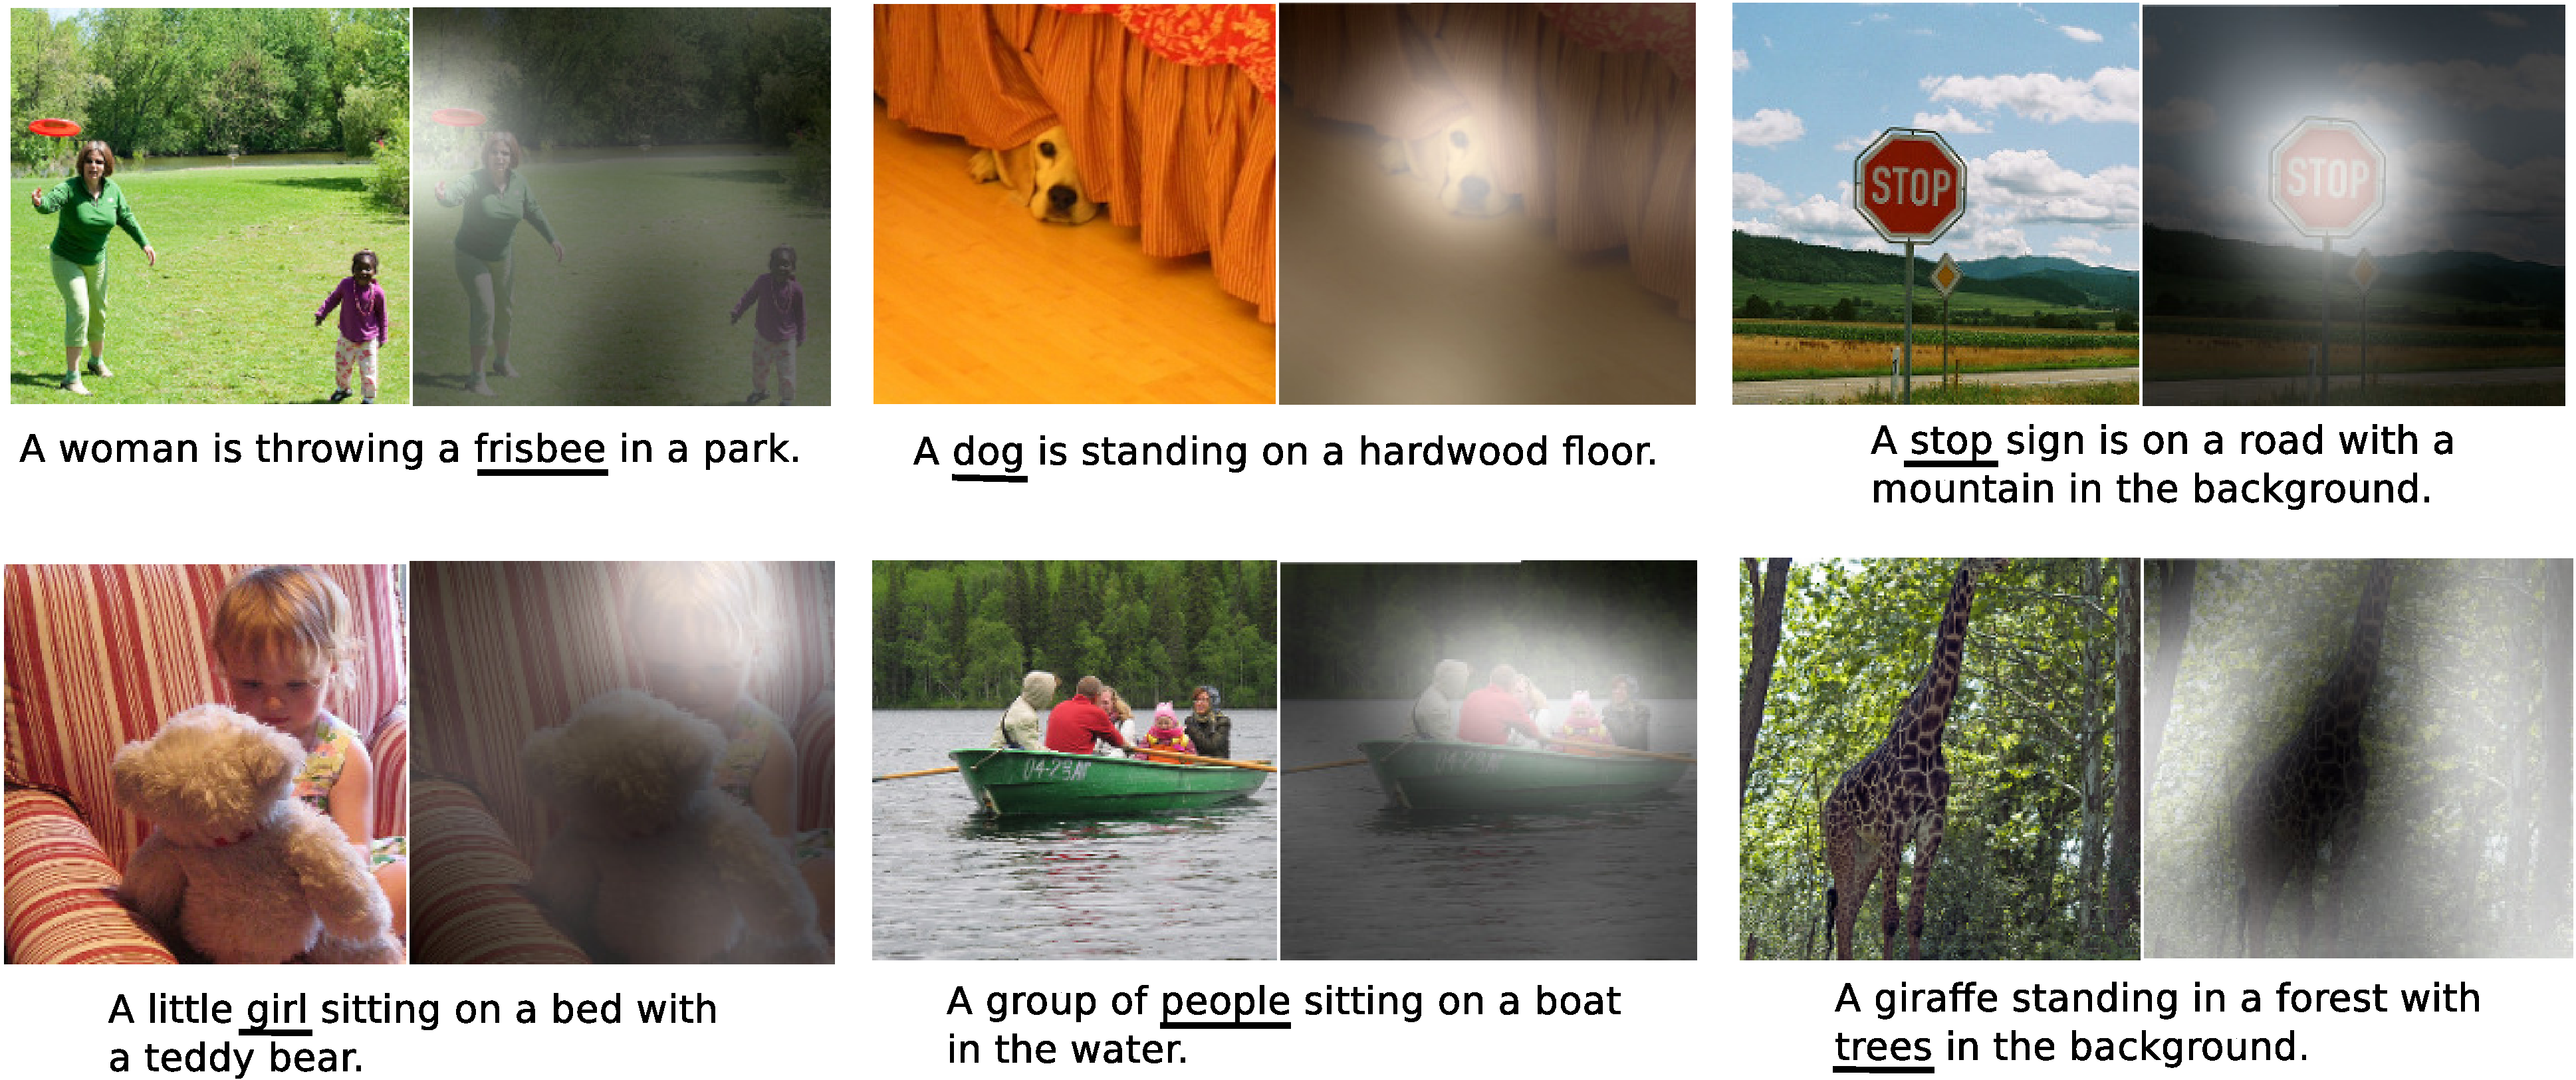
\includegraphics[width=\linewidth]{Images/good_Xu.pdf}
	\caption{Voorbeelden van aandacht op correcte regio. (Wit in de afbeelding is de gefocuste regio, onderlijnde tekst is het overeenkomstige woord.)\cite{Xu2015}}
	\label{fig:attention-example}
\end{figure}

%%% Local Variables: 
%%% mode: latex
%%% TeX-master: "masterproef"
%%% End: 